 \section{Aufbau und Durchführung}
\label{sec:Durchführung}

\begin{figure}
  \centering
  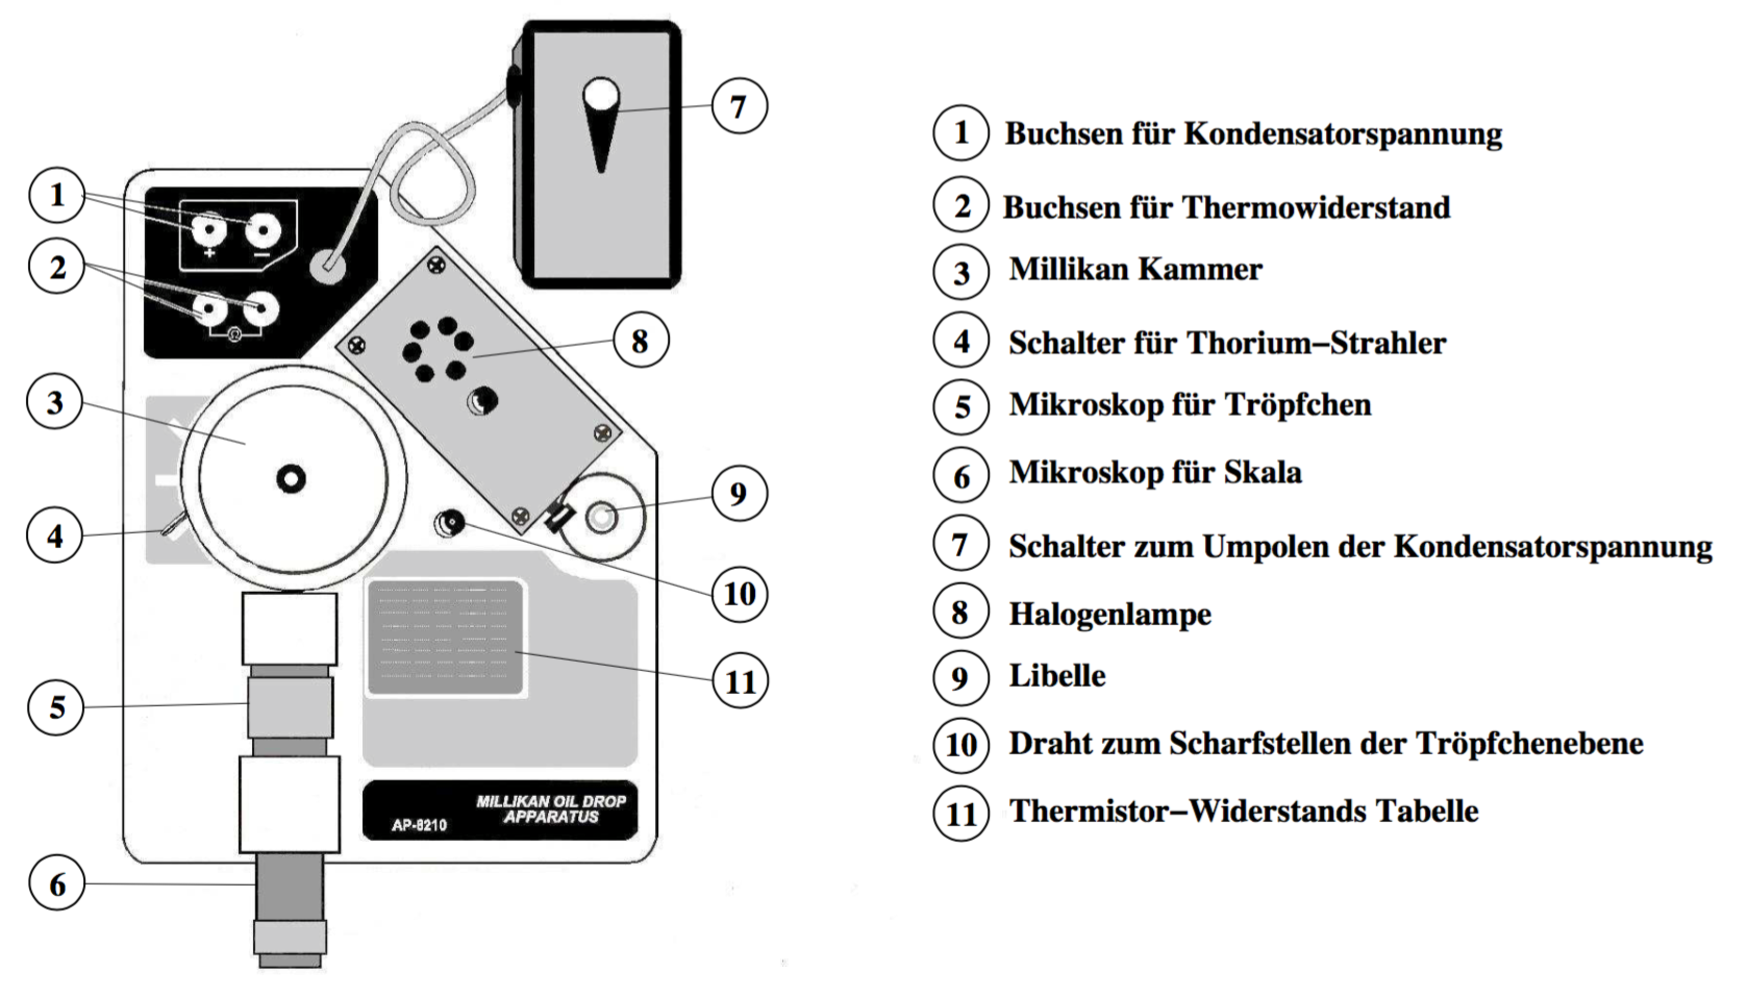
\includegraphics[width = \textwidth]{PicturePerfect/aufbau.pdf}
  \caption{Der genutzte Versuchsaufbau.\cite{anleitung}}
  \label{fig:aufbau}
\end{figure}

In Abbildung \ref{fig:aufbau} ist der Aufbau des Versuchs zu sehen.
Der Teil in dem der Versuch an sich stattfindet ist ein Plattenkondensator mit
Plattenabstand $ d = \SI{7.6250(51)}{\milli\meter}$. In diesen können
mittels einem Zerstäuber die Öltropfen($\rho_\text{Oel} = \SI{886}{\kilogram\per\cubic\metre}$) eingebracht werden. Über eine Vergrößerungsobjektiv
und mit Hilfe einer Halogenlampe können die Tropfen beobachtet werden.
Außerdem ist eine schwache radioaktive Probe ($\ce{^{232}Th}, 8 \mu Ci$) unter dem Kondensator angebracht,
die bei Öffnung der Verdeckung die Luft um die Tropfen ionisiert und so falls nötig zusätzliche Ladung auf das
Tröpfchen bringen kann.
Außerdem kann über den Widerstand des Kondensators und die Abbildungen
\ref{fig:thermistor} und \ref{fig:luftviskositaet} die Viskosität der Luft bestimmt werden.
\begin{figure}
  \centering
  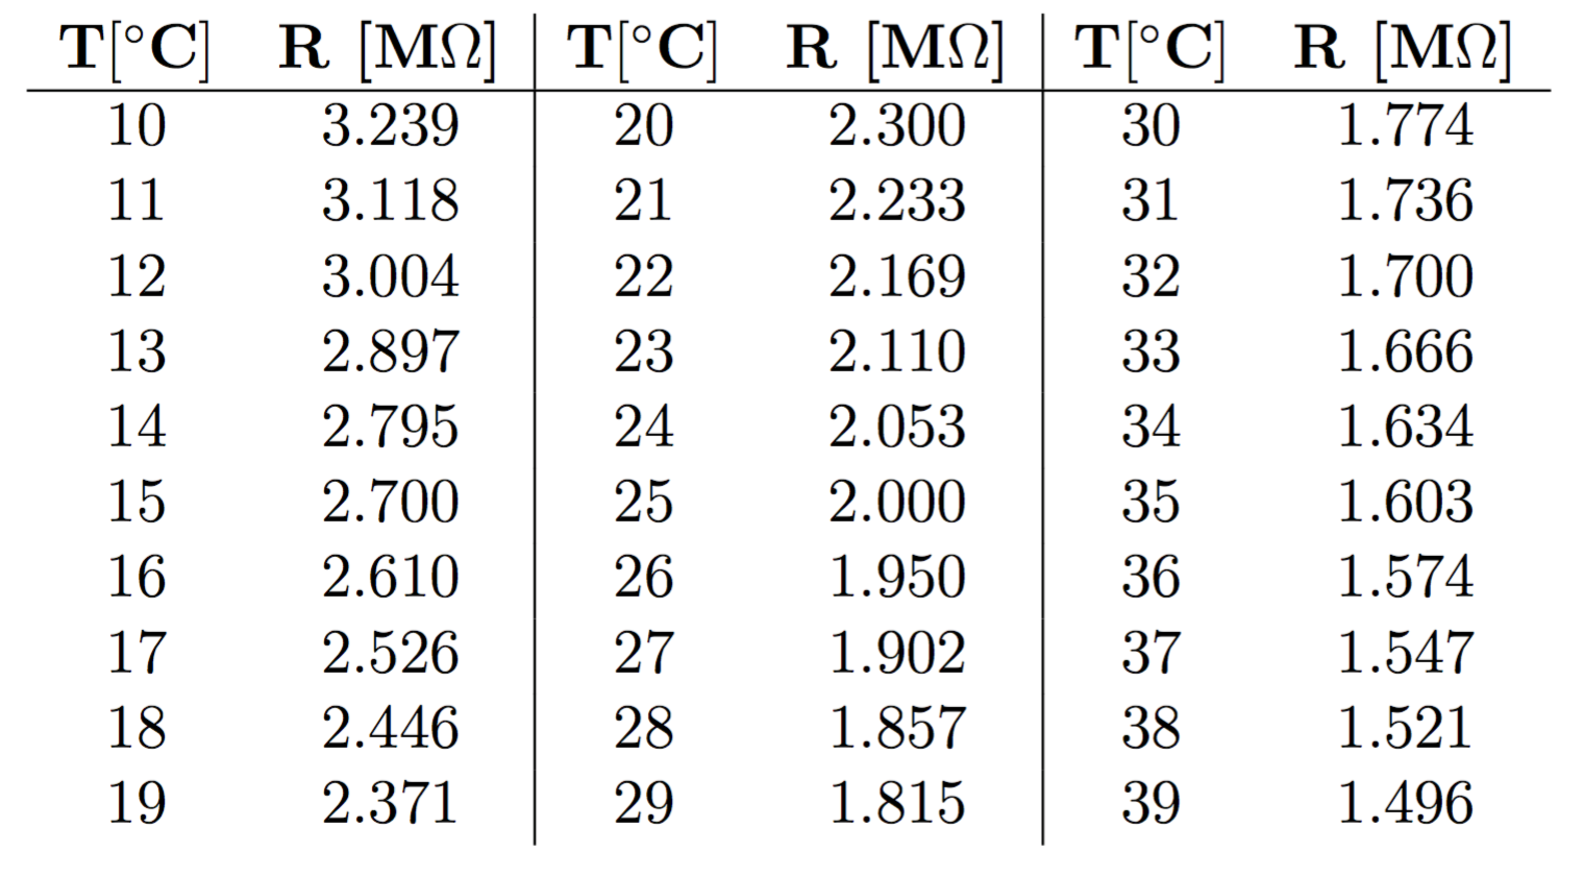
\includegraphics[width = 0.8\textwidth]{PicturePerfect/thermistor.pdf}
  \caption{Thermistor-Widerstandstabelle.\cite{anleitung}}
  \label{fig:thermistor}
\end{figure}
\begin{figure}
  \centering
  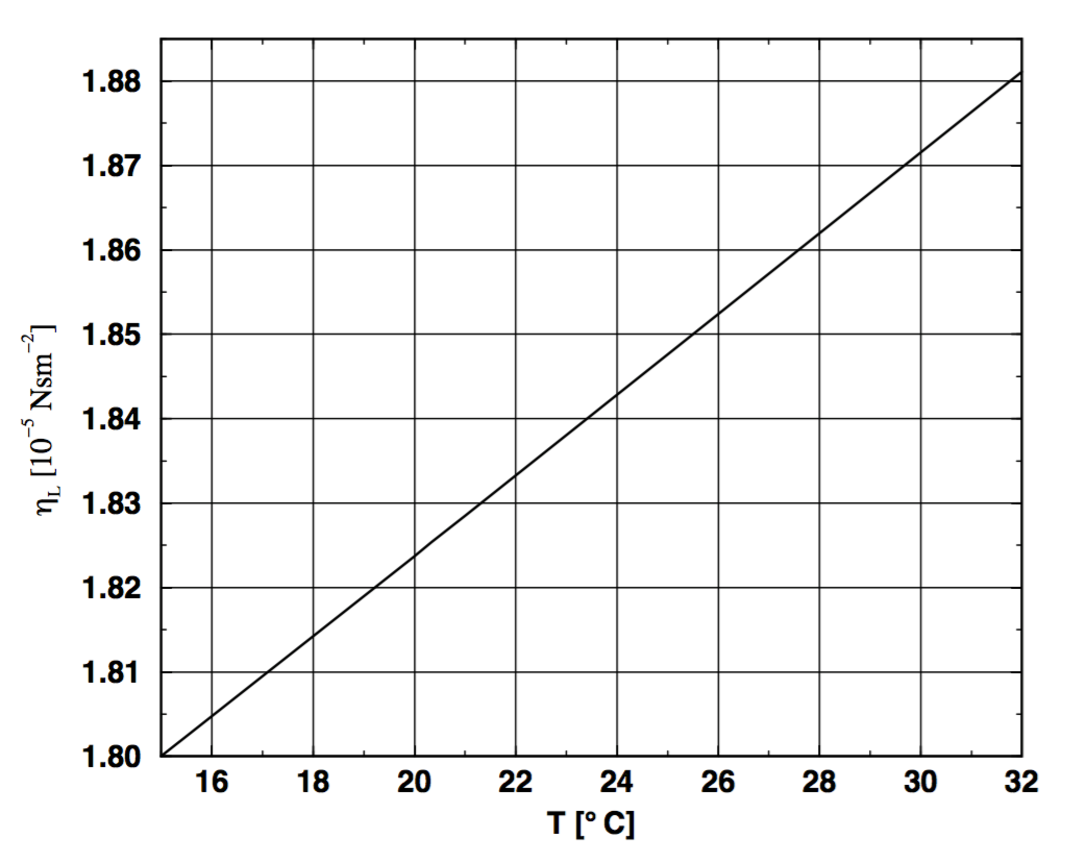
\includegraphics[width = 0.8\textwidth]{PicturePerfect/luftviskositaet.pdf}
  \caption{Viskosität von Luft als Funktion der Temperatur.\cite{anleitung}}
  \label{fig:luftviskositaet}
\end{figure}

\begin{itemize}
  \item Zunächst werden die Tropfen bei ausgeschaltetem Feld eingebracht.
  \item Dann wird ein Tropfen ausgewählt, der bei ausgeschalteter Spannung fällt.
  Außerdem muss er sich durch unterschiedliche Polung der Platten kontrollieren
  lassen.
  \item Gemessen wird nun die Fallgeschwindigkeit $v_0$ ein Mal sowie
  %Steiggeschwindigkeit
  $v_\text{auf}$ und $v_\text{ab}$ vier bis zehn Mal.
  \item Zwischen den Messungen mit verschiedenen Tropfen kann die
  Spannung variiert werden.
  \item Der Widerstand sollte im Verlauf des Versuchs regelmäßig notiert werden.
\end{itemize}
